\documentclass[11pt]{article}
\usepackage{amsfonts}
\usepackage{amsmath}
\usepackage{multicol}
\usepackage[utf8x]{inputenc}
\usepackage{graphicx}
\usepackage{geometry}
\geometry{a4paper, total={170mm, 237mm}, left=20mm, top=20mm}
 
\title{ {\Large \textbf{DÉMONSTRATION AUTOMATIQUE EN COQ}} }
\date{}
\author{Quentin Garchery}

\setlength{\parindent}{0cm}



\usepackage{listings}
\usepackage{color}


\lstdefinelanguage{coq}
{morekeywords={[2]apply,eapply,reflexivity, match, with, end, constr, let, in, forall, change, rewrite, auto, simpl, induction, revert, intro, assumption, split, inversion, destruct, trivial},
keywordstyle={[2]\color{dkblue}},
sensitive=true,
}
\lstset{emph={Lemma, Theorem, Proposition, Qed, Proof, Inductive, Definition, Fixpoint, Ltac, Hint, Resolve, Require, Import, Open, Scope}, emphstyle={\color{mauve}\bf}
}
\definecolor{dkblue}{rgb}{0,0,0.6}
\definecolor{dkgreen}{rgb}{0,0.6,0}
\definecolor{gray}{rgb}{0.5,0.5,0.5}
\definecolor{mauve}{rgb}{0.58,0,0.82}

\lstset{frame=tb,
  language=coq,
  aboveskip=3mm,
  belowskip=3mm,
  showstringspaces=false,
  columns=flexible,
  basicstyle={\small\ttfamily},
  numbers=none,
  numberstyle=\tiny\color{gray},
  keywordstyle=\color{blue},
  commentstyle=\color{dkgreen},
  stringstyle=\color{mauve},
  breaklines=true,
  breakatwhitespace=true,
  tabsize=3
}



\begin{document}




\maketitle
\thispagestyle{empty}

\begin{center}
\normalsize sous la direction de \\

\vspace{3mm}

\begin{multicols}{2}
\large Chantal Keller \\
Maître de Conférences\\
Université Paris-Sud \\

\large Valentin Blot \\
Post-doctorant\\
Université Paris-Sud
\end{multicols}

\vspace{7mm}

\Large{Stage au LRI, Paris-Saclay\\
Université Paris-Sud / CNRS \\}

\vspace{5mm}

\normalsize Mars-Août 2018

\end{center}


\vspace{2cm}


\section{Fiche de synthèse}

\subsection{Contexte général: méthodes formelles}

Les méthodes formelles rassemblent différents logiciels formels qui permettent de formuler des propriétés mathématiques puis de les vérifier. La validité du résultat ne dépend alors que de ce logiciel de vérification. C'est dans ce cadre que G. Gonthier et B. Werner ont prouvé, en Coq, le théorème des quatre couleurs.\medbreak

Les méthodes formelles s'étendent à la preuve de programme: il s'agit alors de vérifier qu'un programme correspond à sa spécification. C'est notamment le cas de Compcert \cite{compcert} qui est un compilateur de code C qui a été certifié en Coq par X. Leroy. La certification d'un programme permet de s'assurer de la robustesse et de la fiabilité de celui-ci. L'importance de la méthode et de la correction des logiciels en général est mise en avant dans le cas des systèmes critiques. En effet, l'échec du premier lancement d'Ariane 5 (1996) est dû à un \textit{bug} logiciel. 

\subsection{Problème étudié}

Parmi ces logiciels formels, on s'intéressera aux assistants de preuve (\ref{assistants}) et aux prouveurs automatiques (\ref{prouveurs}) et plus particulièrement aux interfaces entre un assistant de preuve et différents prouveurs automatiques. De telles interfaces façonnent une preuve à partir du certificat fourni par un des prouveurs automatiques, dans l'objectif d'améliorer l'automatisation de l'assistant de preuve considéré. Ce fonctionnement est celui de Coqhammer \cite{coqhammer} pour l'assistant de preuve Coq et de Sledgehammer \cite{sledgehammer_manual} pour Isabelle. \medbreak

Pendant mon stage, j'ai travaillé sur SMTCoq \cite{smtcoq_code, these_keller} qui sert aussi d'interface à différents prouveurs automatiques mais qui a la particularité de reproduire fidèlement, en Coq, le certificat reçu. Cette approche nécessite la mise en place d'un vérificateur des certificats fournis par les prouveurs automatiques et permet donc, par la même occasion, d'améliorer la confiance que l'on a dans ces outils.\medbreak

Nous aimerions que le développement qui s'appuie sur cette automatisation soit adapté aux assistants de preuve dans lesquels les preuves sont modulaires et peuvent reposer sur des lemmes précédemment démontrés. Nous voudrions aussi pouvoir formaliser une théorie en partant des axiomes de celle-ci puis démontrer automatiquement de nouvelles propriétés de cette théorie.

\subsection{Contribution proposée}

Pendant mon stage, je me suis donc attaché à améliorer l'expressivité de SMTCoq en permettant le développement incrémental d'une théorie. En effet, j'ai ajouté la possibilité de transmettre au prouveur automatique, au sein de SMTCoq, des axiomes ou des lemmes déjà démontrés. Cet ajout s'est traduit par une extension de la logique utilisée et se retrouve dans toutes les étapes intermédiaires de SMTCoq, étapes que j'ai étendues en conséquence. Cette extension a nécessité un développement original: la technique d'encodage des instanciations des lemmes que j'ai utilisée (\ref{processing_forallinst}) permet d'alléger la suite de la vérification. Enfin, j'ai automatisé le procédé de vérification final afin de préserver la facilité d'utilisation de SMTCoq.

\subsection{Arguments en faveur de la validité de la contribution}

En plus des tests présents dans SMTCoq initialement, le code final passe d'autres tests qui requièrent la transmission de lemmes au prouveur automatique. Cela atteste  que l'implémentation de la méthode est valide et induit un gain d'expressivité. J'ai ainsi pu vérifier des propriétés, automatiquement et dans Coq, portant sur: la théorie des groupes, une théorie formalisant les listes d'entiers, des fonctions définies récursivement, etc.

D'autre part, ma contribution respecte le principe sceptique de SMTCoq (\ref{sceptique_autarcique}): le développement et le calcul sont faits principalement en OCaml, en dehors de l'assistant de preuve. Cet aspect donne une meilleure robustesse à SMTCoq face aux changements internes des prouveurs automatiques.


\subsection{Bilan et perspectives}\label{persp}

Les formules acceptées par SMTCoq doivent être exprimées dans le type des booléens et doivent aussi être en forme prénexe. On pourrait améliorer l'expressivité en étendant les cas d'application (\ref{cas_application}) aux formules exprimées dans le type des propositions en Coq.

On pourrait aussi utiliser des méthodes de \textit{machine learning} pour sélectionner les lemmes à envoyer au prouveur automatique comme c'est fait dans Coqhammer et Sledgehammer \cite{hol_selector, coqhammer}. L'avantage étant qu'avec des lemmes pertinents et en petit nombre le prouveur automatique trouve plus rapidement et plus souvent la preuve du théorème en question.

Un autre but que l'on souhaite poursuivre est la certification du logiciel de vérification Why3 \cite{why3_intro}. Puisque Why3 utilise des prouveurs automatiques, cela nécessite de certifier les démonstrations faites par ces prouveurs. Ce sujet est au c\oe ur de celui de ma thèse intitulée "Certification de la génération et la transformation d'obligations de preuves" qui sera encadrée par Claude Marché, Chantal Keller et Andrei Paskevich. À cette occasion, j'utiliserai SMTCoq et je profiterai de l'amélioration de son expressivité due à mon stage. Je pourrai l'améliorer encore en étendant le format des lemmes que l'on peut transmettre à SMTCoq. \medbreak

Ces améliorations de l'expressivité et de l'efficacité combinées avec la facilité d'utilisation et la robustesse de SMTCoq ont pour objectifs d'en faire un outil accessible et de généraliser son utilisation dans les projets développés en Coq.



\newpage
\section{Logiciels utilisés}

\subsection{Assistants de preuve}\label{assistants}

Les assistants de preuve sont des outils puissants qui permettent d'exprimer des théorèmes complexes puis de les vérifier de manière interactive. Ils proposent à un utilisateur de formuler son problème puis de le démontrer, le rôle principal de l'assistant de preuve étant alors de vérifier que la preuve fournie est correcte. Pour une propriété donnée, l'utilisateur doit donc construire une preuve parfaitement rigoureuse et exhaustive de la propriété ce qui peut rendre le processus de vérification long et fastidieux. La confiance accordée à ces outils dépend de la compréhension que l'on peut avoir de son noyau, la vérification étant effectuée par celui-ci. Afin de faciliter cette compréhension, le noyau de l'assistant de preuve Coq est implémenté en OCaml, un langage de haut niveau proche de sa logique. L'accent est mis sur la concision et la clarté du code. \medbreak

Dans la suite nous utiliserons Coq comme assistant de preuve. La logique de son noyau se fonde sur le calcul des constructions inductives \cite{coq_intro}. La sémantique du langage n'est pas donnée en détail dans ce rapport mais les aspects importants seront précisés au moment de leur utilisation. La partie \ref{coq} introduit deux techniques spécifiques à Coq que nous utiliserons. 

\subsection{Prouveurs automatiques}\label{prouveurs}

Les prouveurs automatiques, quant à eux, ne demandent pas de preuves de la part de l'utilisateur. L'effort de certification est alors réduit à la formalisation du problème et dans certains cas le prouveur donne une trace de son exécution appelée certificat. En contrepartie, la logique d'un prouveur automatique est plus limitée et/ou la réponse en temps fini n'est pas garantie. Puisqu'un prouveur automatique doit chercher la preuve du théorème entré, l'efficacité de son implémentation est capitale. Pour cette raison, les prouveurs automatiques sont écrits dans des langages de plus bas niveau tels que C ou C\texttt{++} et font usage de structures mutables complexes. \medbreak

La partie \ref{fonctionnement_prouveurs} détaille le fonctionnement des prouveurs automatiques ainsi que l'utilisation que nous en ferons.


\subsection{SMTCoq}

Une interface entre assistant de preuve et prouveurs automatiques telle que SMTCoq offre les avantages des deux types de logiciels formels décrits ci-dessus. Un autre avantage de SMTCoq est sa modularité: il est en effet possible de prendre en charge d'autres prouveurs automatiques, ceux-ci n'étant pas nécessairement du même type (prouveurs SAT/SMT) et n'ayant pas nécessairement le même format d'entrée ni le même format de sortie. \medbreak


La partie \ref{pres_smtcoq} présente SMTCoq qui est l'objet du stage et qui est un projet actuellement développé par Chantal Keller en collaboration avec l'Université de l'Iowa. Le logiciel SMTCoq est écrit en OCaml et en Coq, langages que j'ai donc utilisés pendant mon stage. \medbreak

Les fragments de code Coq fournis sont encadrés et sont compilables lorsqu'ils sont chargés dans l'environnement de SMTCoq, c'est-à-dire lorsqu'ils sont précédés de:
\begin{lstlisting}[frame=single]
  Require Import SMTCoq Bool.
  Open Scope Z_scope.
\end{lstlisting}
Cela requiert l'installation de SMTCoq, la version contenant ma contribution est disponible à l'adresse:
\begin{align*}
    \texttt{https://github.com/QGarchery/smtcoq-1}
\end{align*}
On préférera la version utilisant native-coq \cite{native-coq} pour des raisons d'efficacité.


\newpage

\section{Techniques de preuves en Coq} \label{coq}

Cette partie présente deux techniques de preuves en Coq qui sont combinées dans SMTCoq: la réflexion calculatoire et la réification.


\subsection{Réflexion calculatoire}

Il est possible d'introduire de nouveaux termes Coq de manière logique à l'aide d'un type  inductif ou de manière calculatoire avec une définition. Nous allons voir que la technique de réflexion calculatoire n'est possible que dans le second cas. Nous commençons par détailler les types inductifs, ce qui permettra de mettre en avant cette différence.

\subsubsection{Types inductifs}

Prenons l'exemple des formules disjonctives booléennes. Ces formules sont des éléments du type inductif \texttt{OrTree} qui a un constructeur \texttt{Bool} pour les feuilles et un constructeur \texttt{Or} pour les nœuds: 

\begin{lstlisting}[frame=single]
Inductive OrTree :=
  Bool (b : bool)
| Or (left: OrTree) (right: OrTree).
\end{lstlisting}

Une première manière de donner l'interprétation des formules est d'utiliser un type inductif:

\begin{lstlisting}[frame=single]
Inductive Interp : OrTree -> Prop :=
  InterpBool :
    Interp (Bool true) 
| InterpOrLeft t1 t2 :
    Interp t1 -> Interp (Or t1 t2) 
| InterpOrRight t1 t2 :
    Interp t2 -> Interp (Or t1 t2).
\end{lstlisting}

Ce type inductif est tel que \texttt{Interp t} signifie que l'interprétation de  \texttt{t} est vraie. Le cas des feuilles \texttt{true} est traité par \texttt{InterBool}. Le constructeur \texttt{InterpOrLeft} nous assure que si l'interprétation de \texttt{t1} est vraie alors, pour tout arbre \texttt{t2}, l'interprétation de \texttt{Or t1 t2} est vraie. Le cas \texttt{InterpOrRight} est similaire.\medbreak

On peut alors faire des preuves sur les éléments de ce type inductif: 
\begin{lstlisting}[frame=single]
Definition t := Or (Or (Bool false) (Bool true)) (Or (Bool false) (Bool false)).

Lemma Interp_t : Interp t.
Proof.
  apply InterpOrLeft.
  apply InterpOrRight.
  apply InterpBool.
Qed.
\end{lstlisting}

\subsubsection{Définitions en Coq et convertibilité}

La réflexion calculatoire repose sur la convertibilité de deux termes: deux termes sont convertibles lorsqu'ils se réduisent vers un même terme. Aussi, à chaque nouvelle définition, la nouvelle constante qui est définie est convertible à sa définition. \medbreak

Plutôt que d'utiliser un prédicat qui prend une formule disjonctive \texttt{t} et qui énonce que l'interprétation de \texttt{t} est vraie, on peut définir une fonction récursive qui calcule l'interprétation et combiner cette fonction avec le prédicat de l'égalité. On peut ensuite montrer que les deux formalisations sont bien équivalentes.  

\begin{lstlisting}[frame=single]
Fixpoint interp (t : OrTree) :=
  match t with
    Bool b => b
  | Or t1 t2 => interp t1 || interp t2
  end.

Proposition Interp_equiv_interp t :
  Interp t <-> interp t = true.
\end{lstlisting}

On a noté \texttt{||} la fonction Coq \texttt{orb} qui implémente la disjonction booléenne.
L'avantage de cette définition de l'interprétation par rapport au type inductif est que, grâce à la convertibilité de \texttt{interp} à sa définition, on a une preuve triviale du lemme précédent.

\begin{lstlisting}[frame=single]
Lemma interp_t : interp t = true.
Proof.
  reflexivity.
Qed.
\end{lstlisting}

En effet, en notant \texttt{a} $\equiv$ \texttt{b} lorsque \texttt{a} est convertible à \texttt{b}, on a:
\begin{align*}
  \texttt{interp t} \equiv \,\, &\texttt{interp (Or (Bool false) (Bool true)) ||}  \\
  \,\, &\texttt{interp (Or (Bool false) (Bool false))} \\
  \equiv \,\, &\texttt{(interp (Bool false) || interp (Bool true)) ||} \\
  \,\,&\texttt{(interp (Bool false) || interp (Bool false))} \\
  \equiv \,\, &\texttt{(false || true) || (false || false)} \\
  \equiv\,\, &\texttt{true}
\end{align*}  

Ce fonctionnement peut être exploité pour construire des preuves qui reposent sur un calcul de convertibilité de termes Coq.


\subsection{Réification} \label{reification}

\subsubsection{\textit{Embeddings}}

La réification est le fait de passer d'un \textit{shallow-embedding} à un \textit{deep-embedding}. Dans le cas du \textit{deep-embedding}, un terme est représenté dans un type de données du langage ce qui met en évidence sa structure. À l'inverse, un \textit{shallow-embedding} du même terme est traduit directement vers sa valeur dans le langage cible. \medbreak

Reprenons l'exemple des formules disjonctives et considérons la formule $ u := (b_1 \vee b_2) \vee (b_3 \vee b4)$. À l'instar de la section précédente, le \textit{deep-embedding} de $u$ est donné dans le type \texttt{OrTree}:
\[\texttt{Or (Or (Bool b1) (Bool b2)) (Or (Bool b3) (Bool b4))}\] 
et son \textit{shallow-embedding} peut être donné en utilisant la disjonction booléenne de Coq: 
\[\texttt{(b1 || b2) || (b3 || b4)} \]
Dans la suite, on s'intéresse au problème de mettre des formules booléennes disjonctives en forme de peigne. Avec \texttt{b1}, \texttt{b2}, \texttt{b3} et \texttt{b4} des termes Coq de type \texttt{bool}, on veut, par exemple, pouvoir passer de
\begin{center}
\texttt{ v := (b1 || b2) || (b3 || b4)}  \hspace{.5cm} à   \hspace{.5cm}  \texttt{v' := b1 || (b2 || (b3 || b4))}
\end{center}
Pour cela, on a besoin de récupérer la structure du booléen \texttt{v}, c'est l'étape de réification. Il s'agit donc de construire, à partir de \texttt{v}, un terme du type \texttt{OrTree} qui a la même structure que \texttt{v}.

\subsubsection{Méthodes}

Il n'est pas possible d'écrire dans le langage du noyau de Coq une fonction qui transforme un terme booléen en forme disjonctive en l'élément du type \texttt{OrTree} correspondant. En effet, le type \texttt{bool} n'ayant que deux constructeurs (\texttt{true} et \texttt{false}), inspecter par \textit{pattern-matching} ne pourra donner que l'un de ces deux constructeurs.\medbreak

Une solution est de travailler directement avec le type de données OCaml des termes Coq. C'est l'approche utilisée par SMTCoq. \medbreak

Le méta-langage des tactiques de Coq, langage non typé, non terminant et implémenté en dehors du noyau, offre la possibilité de manipuler la représentation des termes du noyau. Dans le cas des formules disjonctives, on écrit:
\begin{lstlisting}[frame=single]
Ltac reify A :=  match A with
  | orb ?X ?Y => let rx := reify X in
                    let ry := reify Y in
                    constr:(Or rx ry)
  | ?X => constr:(Bool X) end.

\end{lstlisting}
Le terme \texttt{u := (b1 || b2) || (b3 || b4)} réifié donne bien 
\[\texttt{Or (Or (Bool b1) (Bool b2)) (Or (Bool b3) (Bool b4))}\] 
et on notera que l'interprétation de ce nouveau terme est convertible à \texttt{u}.




\subsubsection{Intérêt et exemple d'utilisation} \label{interet_reification}

L'intérêt de la réification est que la structure du terme réifié est mise en évidence. Il devient alors possible de manipuler explicitement cette structure. \medbreak

Par exemple, sur le type \texttt{OrTree}, il est possible de définir une fonction \texttt{peigne} qui renvoie l'arbre en argument mis sous forme de peigne. Le théorème de correction de cette fonction établit que
\[ \texttt{forall t\,:\,OrTree, interp (peigne t) = interp t} \]
Ce théorème de correction n'est applicable que si on a un terme de la forme \texttt{interp x}. Si \texttt{u} est un terme booléen dont la réification est \texttt{v} (de type \texttt{OrTree}), on peut mettre \texttt{u} sous cette forme en remarquant que $\texttt{interp v}\equiv\texttt{u}$. \medbreak

En combinant tous ces résultats, on peut définir une tactique \texttt{peignify} qui met en forme de peigne les formules disjonctives des deux côtés de l'égalité. Cette tactique permet par exemple de démontrer le lemme suivant: 
\begin{lstlisting}[frame=single]
Lemma or_tree_equality b1 b2 b3 b4:
  (b1 || b2) || (b3 || b4) = b1 || ((b2 || b3) || b4).
Proof.
  peignify. reflexivity.
Qed.
\end{lstlisting}
Cette preuve a un contenu calculatoire: le calcul de la fonction \texttt{peigne} sur la réification des termes booléens de chaque côté de l'égalité. Pour le code complet de cette partie et en particulier le code de la tactique \texttt{peignify}, voir l'annexe A, la preuve de correction est inspirée de \cite{coq_intro}, section 3.3.


\newpage
\section{Prouveurs automatiques} \label{fonctionnement_prouveurs}

\subsection{Utilisation par SMTCoq}

Différents prouveurs automatiques sont mis à la disposition de l'utilisateur de SMTCoq. Parmi ceux-ci, il y a zChaff, un prouveur SAT, c'est-à-dire un prouveur qui résout des problèmes de satisfiabilité de formules booléennes. On trouve aussi des prouveurs SMT (veriT et CVC4) que nous présentons plus en détail dans cette partie.\medbreak 

Pour SMTCoq, les prouveurs automatiques sont vus comme des boîtes noires qui résolvent des problèmes logiques. Plus précisément, SMTCoq interagit avec un prouveur automatique en traduisant le problème dans un format reconnu par celui-ci (\ref{smt-lib}) puis en interprétant sa réponse (\ref{sortie}). Ce fonctionnement est un des intérêts de l'approche sceptique (\ref{sceptique_autarcique}).

\subsection{Prouveurs SMT} \label{smt}

Un problème SMT est un problème de satisfiabilité de formules du premier ordre pour certaines théories prédéfinies. L'algorithme DPLL~\cite{dpll} de résolution des problèmes SAT peut être combiné avec une procédure de décision d'une théorie pour donner un prouveur SMT. Expliquons succinctement le fonctionnement d'une version de cet algorithme DPLL. Nous ne considérerons que la théorie LIA, théorie qui contient les entiers et les symboles d'addition, de soustraction et d'inégalité. On prend en exemple le problème qu'on appellera $pb\_lia$ et qui consiste à satisfaire la formule \[((x + y \leq -3 \wedge y \geq 0) \vee x \leq -3) \wedge x \geq 0\] où $x$ et $y$ sont des entiers. \medbreak

L'algorithme commence par identifier les atomes, c'est-à-dire les sous-formules spécifiques à la théorie LIA. Dans notre exemple cela revient à poser 
\begin{align*}
a &:= \,\, x + y \leq -3 & c &:= \,\,x \leq -3 \\
b &:=\,\, y \geq 0 & d &:= \,\,x \geq 0
\end{align*}
et à chercher si la formule  $((a \wedge b) \vee c) \wedge d$ est satisfiable. Cette étape peut être suivie par une transformation de Tseitin (\ref{tseitin}) afin d'obtenir un problème en Forme Normale Conjonctive (CNF) qui est le format de prédilection des prouveurs SAT. \medbreak

Ensuite, l'algorithme DPLL répète les étapes suivantes:
\begin{itemize}
\item Appeler un prouveur SAT sur la formule. Si ce n'est pas satisfiable, alors l'algorithme répond que le problème n'est pas satisfiable.
\item Dans le cas contraire, le prouveur SAT donne une instanciation qui satisfait toutes les formules. La formule de l'exemple est satisfiable, une instanciation pourrait être:
  $a \, \wedge\,\neg b \, \wedge c\, \wedge \,d$,
ce qui signifie que toutes les variables booléennes sont à $true$ sauf $b$ qui est à $false$.
\item Appeler la procédure de décision pour vérifier que l'instanciation est valide dans la théorie. Si c'est le cas, l'algorithme renvoie que le problème est satisfiable.
\item Sinon, rajouter la négation de l'instanciation à la liste des formules et recommencer. C'est le cas de notre exemple: il n'est pas possible, dans la théorie LIA, d'avoir à la fois $x \leq -3$ et $x \geq 0$. À la fin de cette étape, le problème est donc ramené à la satisfiabilité des deux formules suivantes:
  \begin{align*}
    ((a \wedge b) \vee c) \wedge d \\
    \neg a \vee b \vee \neg c \vee \neg d.
  \end{align*}
\end{itemize}

Cet algorithme termine puisqu'à chaque répétition des étapes ci-dessus une nouvelle instanciation des atomes n'est plus possible et qu'il y a un nombre fini de telles instanciations. 

\subsection{Format d'entrée, le langage SMT-LIB} \label{smt-lib}

Le langage SMT-LIB a vocation à être un format d'entrée commun à différents prouveurs SMT tels que veriT. Ce langage offre donc un cadre pour faire des comparaisons de prouveurs SMT. La définition du langage \cite{smtlib} donne des indications sur la sémantique que doivent avoir certaines constructions du langage.\medbreak

Le problème $pb\_lia$ de la section précédente peut être écrit dans le langage SMT-LIB:
\begin{lstlisting}[frame=no]
(set-logic QF_LIA)
(declare-fun x () Int)
(declare-fun y () Int)
(assert (and (or (and (<= (+ x y) (- 3)) (>= y 0)) (<= x (- 3))) (>= x 0)))
(check-sat)
(exit)
\end{lstlisting}
On appelle assertion une formule contenue dans une ligne d'un fichier SMT-LIB commençant par $assert$: la formule $((x + y \leq -3 \wedge y \geq 0) \vee x \leq -3) \wedge x \geq 0$ est une assertion dans le fichier ci-dessus.


\subsection{Format de sortie, les certificats de veriT} \label{sortie}

Lorsqu'on appelle un prouveur automatique sur un fichier SMT-LIB, si la conjonction des assertions est satisfiable, le prouveur renvoie $sat$. Si la conjonction des assertions n'est pas satisfiable, le prouveur renvoie $unsat$ et fournit un fichier de certificat expliquant la raison de cette non-satisfiabilité. Le format de ce fichier de certificat peut varier en fonction du prouveur SMT considéré. \medbreak

Dans la suite de cette section nous nous intéressons aux certificats du prouveur SMT veriT. Ceux-ci utilisent des clauses, une clause étant une disjonction de formules écrite sous forme de liste. Nous noterons $(f_1 \,\,  ... \,\, f_n)$ la clause contenant les formules $f_1$, ..., $f_n$. La clause vide, notée $()$, représente l'absurde. Les certificats de veriT sont constitués d'une suite de règles de la forme: 
\[id:(typ \,\, cl \,\, dep)\] 
où $id$ est un entier qui identifie la règle, $typ$ est le type de la règle, $cl$ est une clause qu'on appelle résultat de la règle et $dep$ liste toutes les dépendances de la règle.  Ainsi, montrer que le problème n'est pas satisfiable revient à obtenir une suite de règles dont le résultat de l'une d'entre elles est la clause vide. Une règle peut utiliser le résultat d'une autre règle identifiée par $id$, dans ce cas sa liste de dépendances contient l'identifiant $id$.

\subsubsection{Règle $input$}

Les règles de type $input$ sont des règles qui établissent les hypothèses du problème et correspondent aux assertions du fichier SMT-LIB. Par exemple, la règle 
\[ 1:(input \,\, (x \geq 0)) \]
est utilisée dans le cas où on suppose que $x$ est un entier positif. Cette règle (et les règles $input$ en général) ne dépend pas du résultat d'autres règles.\medbreak

\subsubsection{Règle $resolution$}

Pour manipuler ces clauses, veriT peut utiliser une règle $resolution$. La règle de résolution appliquée à deux clauses donne une nouvelle clause contenant toutes les formules de ces deux clauses sauf les formules qui ont leur négation dans l'autre clause. Par exemple, la résolution de $a \vee b$ et de $\neg a \vee \neg c$ donne $b \vee \neg c$. Grâce à cette règle, on peut montrer que le problème qui suppose l'existence d'un entier $x$ tel que $x \geq 0$ et $\neg (x \geq 0)$ n'est pas satisfiable: 
\begin{align*}
1&:(input \,\, ( x \geq 0)) \\
2&:(input \,\, (\neg (x \geq 0))) \\
3&:(resolution \,\,() \,\,1\,\, 2)
\end{align*}

Une règle de résolution peut avoir plus de deux dépendances. Son résultat est alors défini récursivement à partir de ceux des règles de résolution appliquées à deux clauses. Par exemple, le résultat de la règle \[4:(resolution \,\,(B) \,\,1\,\, 2\,\,3) \]
est le même que celui de la règle $5$ lorsque la règle ci-desus est remplacée par les règles
\begin{align*}
4&:(resolution \,\,(A) \,\,1\,\, 2) \\
5&:(resolution \,\,(B) \,\,4\,\, 3) 
\end{align*}

\subsubsection{Règles $not\_implies0$ et $not\_implies1$} \label{not_implies}
La règle $not\_implies0$ implémente la règle logique qui donne $A$ à partir de $\neg (A \Rightarrow B)$ et $not\_implies1$ implémente la règle logique qui donne $\neg B$ à partir de $\neg (A \Rightarrow B)$. \medbreak

Ces règles dépendent donc du résultat d'une autre règle qui doit nécessairement être une clause de la forme $(\neg (X \Rightarrow Y))$. Les résultats des règles $not\_implies0$ et $not\_implies1$ sont alors respectivement $(X)$ et $(\neg Y)$. Cette règle nous permet de montrer que la formule $\neg (A \Rightarrow A)$ n'est pas satisfiable:
\begin{align*}
  1&:(input\,\, (\neg ( A \Rightarrow A))) \\
  2&:(not\_implies0\,\, (A)\,\, 1) \\
  3&:(not\_implies1\,\, (\neg A) \,\,1) \\
  4&:(resolution\,\, ()\,\, 2\,\, 3)
\end{align*}


\section{Présentation de SMTCoq} \label{pres_smtcoq}

\subsection{SMTCoq, une interface sceptique entre Coq et les prouveurs automatiques}\label{sceptique_autarcique}

Pour améliorer l'automatisation de Coq et y intégrer l'utilisation de prouveurs automatiques, il y a principalement deux approches.

\begin{multicols}{2}
\begin{center}
Approche autarcique\\
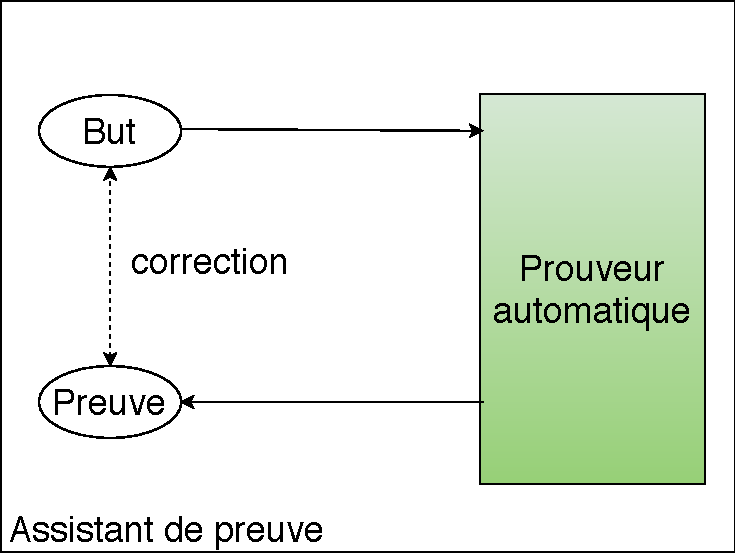
\includegraphics[height=5cm]{1_Autarcique.pdf}\\
Approche sceptique\\
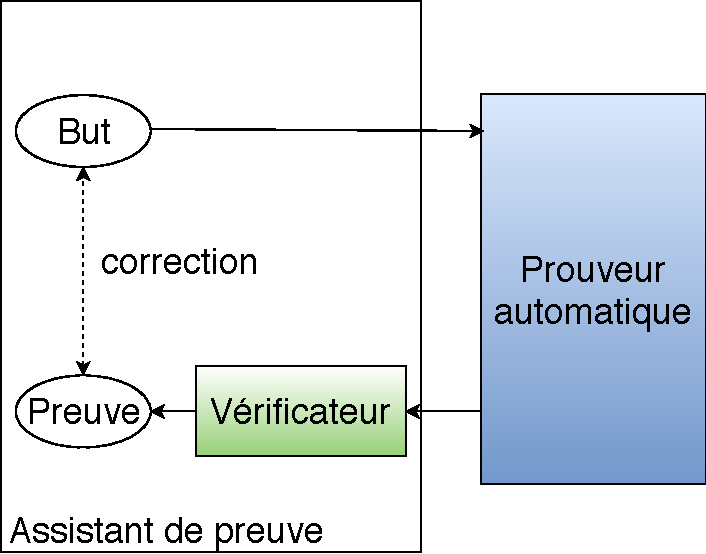
\includegraphics[height=5cm]{2_Sceptique.pdf}\\

\end{center}
\end{multicols}

L'approche autarcique consiste à vérifier le code du prouveur automatique à l'intérieur de l'assistant de preuve. L'avantage de cette méthode est qu'une fois cette vérification faite, on sait que chaque appel du prouveur automatique nous renverra une preuve correcte. \medbreak

Dans l'approche sceptique, le certificat renvoyé par le prouveur automatique est vérifié à chaque appel de celui-ci. Cette approche, utilisée par SMTCoq, ne permet pas de garantir la complétude du système: certains buts valides ne sont pas démontrés, notamment lorsque le prouveur automatique renvoie un certificat erroné ou que la reconstruction de la preuve par SMTCoq n'est pas possible. En revanche, cette approche ne fige pas l'implémentation du prouveur automatique puisque ce n'est pas son code qui est vérifié mais sa réponse. Un autre avantage est que l'effort de certification est plus restreint: pour un certificat fixé, il faut vérifier que celui-ci correspond bien à une preuve du but.

\subsection{Fonctionnement de SMTCoq}

\subsubsection{Amélioration de l'automatisation}\label{smtcoq_automatisation}

Chacune des tactiques Coq définies par SMTCoq invoque un prouveur automatique différent: zChaff, CVC4 ou veriT. Ces tactiques permettent à l'utilisateur Coq de faire appel à un prouveur automatique pour résoudre le but courant et donc de profiter de l'automatisation du prouveur. \medbreak



Les prouveurs automatiques fournissent un certificat uniquement dans le cas où le problème n'est pas satisfiable (\ref{sortie}). Pour exploiter ce fonctionnement, SMTCoq envoie la négation du but au prouveur automatique. La preuve ne peut être reconstruite que dans le cas où la réponse est $unsat$ et est accompagnée d'un fichier de certificat. Ce fichier prouve que la négation du but mène à l'absurde. Autrement dit, on obtient une preuve de la double négation du but. Afin de pouvoir en déduire le but, SMTCoq requiert des formules exprimées dans les booléens. En effet, le type des booléens relève de la logique classique alors que le type des propositions de Coq est intuitionniste. 

\begin{center}
    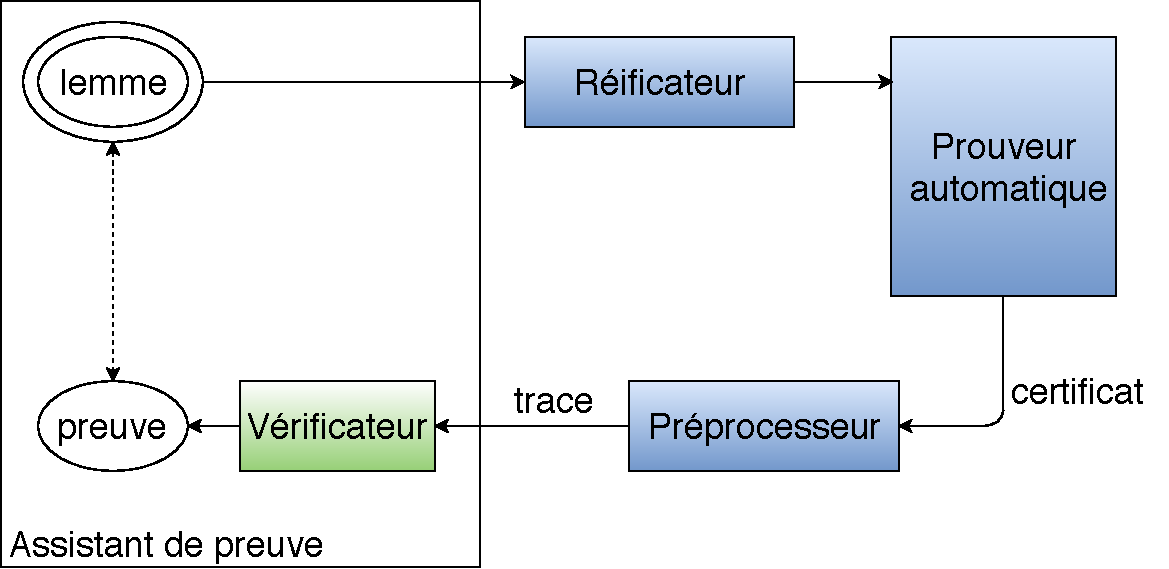
\includegraphics[height=5cm]{Automatisation.pdf}
\end{center}

La première étape est la réification, l'énoncé du lemme est traduit en un AST appartenant au type des formules acceptées par SMTCoq. Cet AST est traduit en un fichier SMT-LIB qui est donné en entrée au prouveur automatique. En cas de succès de ce prouveur, on obtient un fichier de certificat. Ce fichier de certificat est ensuite traduit par le préprocesseur dans un format adapté au vérificateur de SMTCoq. Ce dernier rejoue la preuve en Coq (voir partie \ref{transformation_certif}).


\subsubsection{Amélioration de la confiance} \label{smtcoq_confiance}

Dans la suite on s'attachera principalement à développer l'aspect automatisation de Coq mais SMTCoq propose également une commande de reconstruction d'une preuve effectuée par un prouveur automatique.

\begin{center}
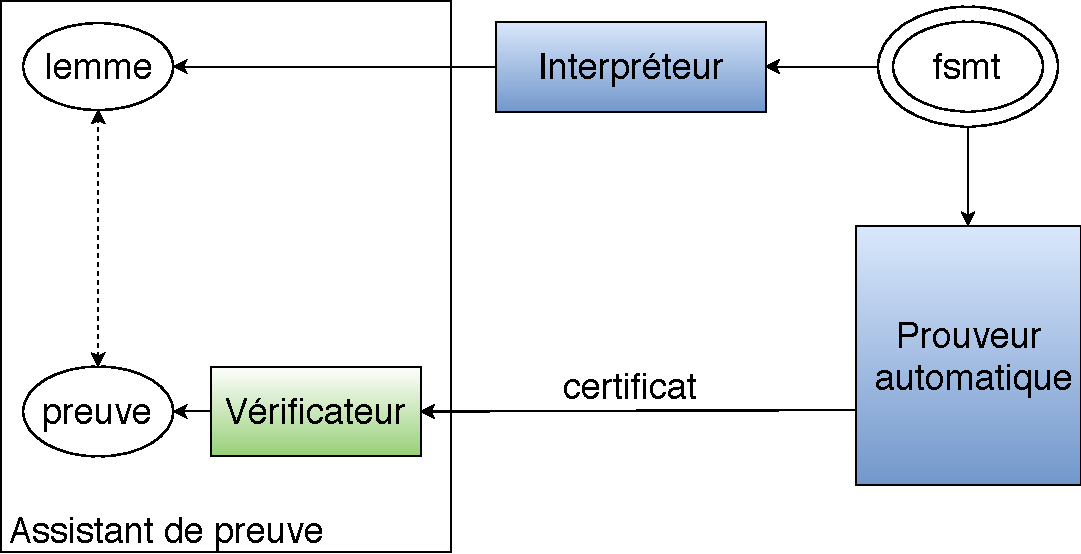
\includegraphics[height=5cm]{Confiance.pdf}
\end{center}

Cette commande prend en paramètre un fichier \textit{fsmt} décrivant le lemme (typiquement écrit en SMT-LIB) et le certificat fourni par un prouveur automatique. Le lemme Coq est reconstruit à l'aide de l'interpréteur de SMTCoq et la preuve est reconstruite grâce au vérificateur. Une fois la reconstruction faite, la vérification que la preuve correspond bien au lemme est laissée à Coq. \medbreak

Puisqu'un nouveau lemme Coq est créé, l'utilisateur peut vérifier que c'est bien le but qu'il voulait prouver. Ainsi, la confiance dans les prouveurs automatiques est améliorée: on peut vérifier la réponse du prouveur.


\subsubsection{Cas d'application de SMTCoq} \label{cas_application}

Dans les deux cas, les formules acceptées sont les formules logiques booléennes en forme prénexe. Les formules atomiques doivent aussi être décidables. Les théories suivantes et leurs combinaisons sont implémentées dans SMTCoq: arithmétique linéaire sur $\mathbb{Z}$, égalité et fonctions non interprétées, auxquelles s'ajouteront la théorie des vecteurs de bits et la théorie des tableaux. 

\subsection{Utilisation de SMTCoq}

\subsubsection{La tactique \texttt{verit}}

Afin d'améliorer l'automatisation de Coq (\ref{smtcoq_automatisation}), SMTCoq définit la tactique \texttt{verit}. Cette nouvelle tactique permet de résoudre automatiquement les buts dans les booléens en forme prénexe. On reprend l'exemple de la partie \ref{fonctionnement_prouveurs}. En utilisant les fonctions booléennes de Coq, \texttt{negb} pour la négation, \texttt{\&\&} pour la conjonction, et \texttt{>=?} et \texttt{<=?} pour les inégalités larges, le problème $pb\_lia$ devient :

\begin{lstlisting}[frame=single]
Lemma pb_lia : 
  forall x y,
    negb ( ((x+y <=? - (3)) && (y >=? 0) || (x <=? - (3))) && (x >=? 0)).
Proof.
    verit.
Qed.
\end{lstlisting}

La tactique \texttt{verit} commence par introduire les variables quantifiées universellement en tête de formule (dans l'exemple ce sont \texttt{x} et \texttt{y}) puis s'attend à ne pas avoir d'autres quantificateurs. C'est ensuite la négation de la formule qui est envoyée à veriT. La reconstruction de la preuve ne peut avoir lieu que si veriT renvoie $unsat$ ainsi qu'un fichier de certificat.

\subsubsection{La commande de reconstruction}

La commande \texttt{Verit\_Theorem} nous permet de créer un terme Coq à partir du certificat fourni par veriT appelé sur le problème $pb\_lia$. On obtient alors le terme Coq \texttt{pb\_lia}:
\begin{center}
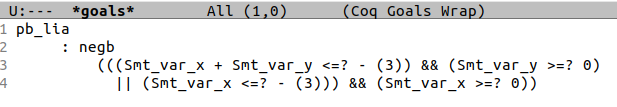
\includegraphics[height=2cm]{pb_lia.png}
\end{center}

On notera que ce terme représente bien la négation de la formule énoncée dans le fichier SMT-LIB, ce qui nous permet de vérifier la réponse du prouveur automatique (\ref{smtcoq_confiance}). 



\section{Transformation de certificats} \label{transformation_certif}

Nous avons vu que c'est grâce à un procédé de réification (\ref{reification}) que l'on peut transmettre le but Coq initial au prouveur automatique. Nous allons maintenant voir comment la réponse du prouveur automatique, le fichier de certificat, peut être transformée en un terme de preuve Coq.

\subsection{Des certificats de toutes les couleurs} \label{des_certificats}

La tactique \texttt{verit} interprète le fichier de certificat \textit{tcertif} fourni par le prouveur automatique en un terme Coq \textit{ccertif}, ce qui permet de construire une preuve du but initial. 

\begin{center}
\begin{tabular}{ |c||c|c|c| } 
 \hline
 Format & Fichier texte & Code OCaml & Code Coq \\ 
 \hline
 Appellation & \textit{tcertif} & \textit{ocertif} & \textit{ccertif} \\ 
 \hline
 Composant & \textit{trule} & \textit{orule} & \textit{crule} \\ 
 \hline
\end{tabular}
\end{center}

Cette interprétation passe par une étape intermédiaire \textit{ocertif} écrite en OCaml. Cette étape a plusieurs avantages. En premier lieu, elle permet d'utiliser les outils de \textit{parsing} du fichier de certificat ($ocamllex$, $ocamlyacc$). Par ailleurs, en utilisant la représentation OCaml des termes Coq, la traduction d'un \textit{ocertif} en un \textit{ccertif} est facilitée. Enfin, les \textit{ocertif} sont définis dans un format facilement manipulable ce qui permet d'appliquer des adaptations (\ref{lien_parsing} et \ref{processing_forallinst}), des simplifications (\ref{regroupement}) ou encore des optimisations (\ref{alloc}).

\subsection{Transformation de Tseitin et \textit{hash consing}} \label{tseitin}

\subsubsection{Motivations}

La transformation de Tseitin d'une formule donne une formule équisatisfiable qui est en CNF en introduisant de nouvelles variables booléennes. L'avan\-tage de cette transformation est que sa complexité est linéaire en temps comme en espace. En comparaison, l'utilisation des lois de De Morgan pour obtenir une formule en CNF a une complexité en pire cas exponentielle. Le principe de cette transformation est d'introduire de nouvelles variables pour toutes les sous-formules, ce qui correspond au \textit{hash consing} qui est fait par SMTCoq \cite{smtcoq_code}. Cette étape intervient au moment du \textit{parsing}, c'est-à-dire au moment du passage d'un \textit{tcertif} à un \textit{ocertif}. Du point de vue de SMTCoq, ce procédé signifie un gain en espace (les sous-formules ne sont pas répétées) et un gain en temps (les comparaisons de formules deviennent des comparaisons d'entiers).


\subsubsection{Fonctionnement}

La transformation commence par nommer toutes les sous-formules en partant des feuilles. La nouvelle formule à satisfaire est alors la conjonction de la variable représentant toute la formule et de formules additionnelles qui garantissent que les nouvelles variables sont équivalentes aux sous-formules qu'elles représentent. \medbreak

On reprend l'exemple de la partie \ref{fonctionnement_prouveurs}. En nommant les atomes on avait obtenu la formule $((a \wedge b) \vee c) \wedge d$. On introduit également $e$ pour la sous-formule $a \wedge b$, $f$ pour la sous-formule $e \vee c$ et $g$ pour la sous-formule $f \wedge d$ qui est en fait toute la formule. La formule transformée devient donc $g \wedge D_e \wedge D_f \wedge D_g$ où les $D_\alpha$ sont des formules qui nous assurent que la variable $\alpha$ est équivalente à la formule qu'elle représente. On a par exemple $D_e = (\neg a \vee \neg b \vee e) \wedge (\neg e \vee a) \wedge (\neg e \wedge b)$ qui nous assure que la variable $e$ est équivalente à $a \wedge b$. \medbreak

Dans SMTCoq, au lieu de rajouter les formules $D_\alpha$, les sous-formules sont enregistrées dans un tableau: la variable $e$ est un indice du tableau et le tableau contient, à cet indice, la formule représentée par $e$ ($a \wedge b$ dans notre exemple).

\subsection{Le vérificateur}

Le vérificateur de SMTCoq contient un type inductif \textit{crule} qui représente les \textit{trule} ainsi qu'une fonction \texttt{checker}. Nous allons définir ces termes Coq, voir comment ils implémentent la sémantique des certificats de veriT (\ref{sortie}) et comment ils sont utilisés pour produire le terme de preuve.


\subsubsection{Le type inductif \textit{crule}}\label{regroupement}


Chaque constructeur du type inductif \textit{crule} représente une famille de  \textit{trule}. Le constructeur \texttt{Res} ne représente que la règle $resolution$ mais d'autres constructeurs peuvent représenter différentes règles en fonction de leurs paramètres. Par exemple, le constructeur \texttt{ImmBuildProj} regroupe les règles $not\_implies0$ et $not\_implies1$ (\ref{not_implies}) et contient aussi un paramètre entier qui vaut \texttt{0} ou \texttt{1} et qui indique quelle est la \textit{trule} représentée. Ce regroupement de règles au fonctionnement similaire permet, dans la suite, de simplifier le traitement de ces règles. \medbreak

On appellera \textit{ccertif} le type des certificats en Coq représentés par des listes de \textit{crule}.


\subsubsection{La fonction récursive \texttt{checker}} \label{checker}

Pour enregistrer le résultat des règles précédentes on utilise un tableau de clauses appelé état, le premier emplacement ayant pour indice \texttt{1}. On rappelle qu'une clause représente la disjonction d'une liste de formules et est notée  entre parenthèses. La fonction \texttt{checker} implémente l'application des règles du certificat et modifie donc l'état à chaque nouvelle \textit{crule} rencontrée. Plus précisément, \texttt{checker} est une fonction Coq qui est définie récursivement sur son paramètre de type \textit{ccertif} et qui a aussi un paramètre état. Le résultat des \textit{crule} suit le fonctionnement des $trule$. Par exemple le résultat de \texttt{ImmBuildProj 0 1} est $(X)$ si le premier emplacement du tableau d'état est de la forme $(\neg (X \Rightarrow Y))$. À chaque appel de \texttt{checker}, une nouvelle \textit{crule} est consommée, son résultat est enregistré dans l'état.\medbreak

Il n'y a pas de \textit{crule} correspondant à la règle $input$: l'état est initialisé avec le résultat de la règle $input$. Dans un premier temps nous considérerons que la taille du tableau est égale au nombre de règles du \textit{tcertif}.\medbreak

Lorsque toute la liste \textit{ccertif} a été consommée, \texttt{checker} renvoie \texttt{true} si le dernier emplacement modifié de l'état contient la clause vide et \texttt{false} sinon.

\subsubsection{Théorème de correction}

Sur le type des formules, SMTCoq définit une fonction \texttt{interp} qui inverse la réification (\ref{interet_reification}). Le vérificateur repose sur le théorème de correction qui nous assure que pour tout \textit{ccertif} \texttt{cc} et toute formule \texttt{f}, si le tableau d'état \texttt{t} est initialisé comme décrit précédemment,  alors: 
\[ \texttt{checker cc t = true -> negb (interp f)} \]
 Une fois celui-ci démontré, la preuve du but initial est obtenue en appliquant le théorème de correction puis la réflexivité de l'égalité. En effet, si \texttt{checker cc t} est convertible à \texttt{true}, alors l'hypothèse \texttt{checker cc t = true} est convertible à \texttt{true = true}.

\subsubsection{Preuve du théorème de correction} \label{preuve_correction}

On dit qu'une clause est valide lorsque son interprétation est prouvable. La preuve du théorème de correction utilise la proposition \texttt{step\_checker\_correct} qui s'énonce ainsi: si toutes les clauses du tableau d'état sont valides alors une étape de \texttt{checker} modifie ce tableau en un tableau dont toutes les clauses sont valides. Il suffit en fait de vérifier que la nouvelle clause générée par \texttt{checker} est valide. \medbreak

À partir de cette proposition on obtient une preuve du théorème de correction. Donnons les grandes étapes de la preuve de ce théorème. Pour prouver $\texttt{checker cc t = true -> negb (interp f)}$, on suppose \texttt{interp f} et \texttt{checker cc t = true}. Initialement, l'état ne contient donc que des clauses valides (tous les emplacements du tableau contiennent \texttt{f}). D'après \texttt{step\_checker\_correct}, cette propriété est conservée par la fonction \texttt{checker}. Si de plus \texttt{checker} renvoie \texttt{true} cela veut dire qu'il y a la clause vide dans le dernier tableau d'état. L'interprétation de la clause vide nous conduit à une contradiction.


\subsubsection{Exemple de l'identité} \label{id_exemple}

Considérons la proposition Coq suivante où \texttt{implb} est l'implication booléenne:
\begin{lstlisting}[frame=single]
  Proposition identity A : implb A A.
\end{lstlisting}

Lorsqu'on applique \texttt{verit}, puisque c'est la négation du but qui est envoyée, le prouveur automatique nous renvoie le \textit{tcertif} de \ref{not_implies}. Celui-ci est traduit par SMTCoq en un \textit{ccertif}
\[ \texttt{cc := [ImmBuildProj 0 1; ImmBuildProj 1 1; Res 2 3] } \]
et l'état est initialisé en un tableau 
\[\texttt{t := [|nid; nid; nid; nid|]}\] 
où \texttt{nid} est la clause $(\neg (A \Rightarrow A))$.
Le calcul de \texttt{checker} est alors:
\begin{align*}
  \texttt{checker cc t}\,\, &\equiv \,\, \texttt{checker [ImmBuildProj 1 1; Res 2 3] [|nid; }(A)\texttt{; nid; nid|]} \\
    &\equiv \,\, \texttt{checker [Res 2 3] [|nid; }(A)\texttt{; }(\neg A)\texttt{; nid|]} \\
    &\equiv \,\, \texttt{checker [] [|nid; }(A)\texttt{; }(\neg A)\texttt{; }()\texttt{|]} \\
    &\equiv \,\, \texttt{true}
\end{align*}
En appliquant le théorème de correction, on obtient \texttt{negb (interp (}$\neg (A \Rightarrow A)$\texttt{))} qui est convertible à \texttt{negb (negb (implb A A))}. Cette proposition est bien équivalente à \texttt{implb A A}.

\subsection{Le préprocesseur}

La transformation des certificats passe par une étape intermédiaire (\ref{des_certificats}) qui nous permet d'améliorer l'efficacité de la transformation et facilite la traduction des certificats dans un format adapté au vérificateur. Nous donnons le format des certificats de cette étape puis une optimisation rendue possible par cette étape.

\subsubsection{Le type OCaml \textit{orule}}

 Les \textit{orule} sont des enregistrements constitués, en plus du code OCaml d'une \textit{crule}, de méta-données qui permettent l'implémentation d'un préprocesseur efficace.

\subsubsection{Allocation dans le tableau d'état} \label{alloc}

On remarque que dans l'exemple de l'identité (\ref{id_exemple}), le tableau d'état n'a pas besoin d'être de taille 4: 2 emplacements suffisent pour ce certificat. De manière générale, on peut réduire l'espace mémoire utilisé en calculant le nombre maximal de clauses à retenir à chaque étape de \texttt{checker}, c'est ce que fait la fonction $alloc$. Cette fonction assigne aussi, pour chaque règle, un emplacement dans l'état où enregistrer son résultat. Ce paramètre de position est noté au début des \textit{crule}, de sorte que lorsque \texttt{checker} rencontre \texttt{ImmBuildProj 1 0 2}, le premier emplacement de l'état est modifié en $(X)$ si le deuxième emplacement de l'état contient $\neg(X \Rightarrow Y)$. Puisque les emplacements des clauses sont modifiés, il faut aussi modifier les dépendances des règles. Enfin, \texttt{checker} prend un paramètre qui indique quelle est la position du résultat de la dernière règle, celui-ci n'étant pas nécessairement au dernier emplacement de l'état comme précédemment. En initialisant \texttt{t} à \texttt{[|nid; nid|]} et en posant \texttt{cc := [ImmBuildProj 1 0 2; ImmBuildProj 2 1 2; Res 1 1 2]}, on a :
\begin{align*}
  \texttt{checker cc t 1} \,\,&\equiv \,\, \texttt{checker [ImmBuildProj 2 1 2; Res 1 1 2] [|}(A)\texttt{; nid|] 1} \\
    &\equiv \,\,\texttt{checker [Res 1 1 2] [|}(A)\texttt{; }(\neg A)\texttt{|] 1} \\
    &\equiv \,\,\texttt{checker [] [|}()\texttt{; }(\neg A)\texttt{|] 1} \\
    &\equiv \,\,\texttt{true}
\end{align*}


\section{Préprocesseur pour les lemmes quantifiés}

Dans cette partie on commence par donner la forme générale des certificats de veriT dans le cas des lemmes quantifiés universellement. On explique ensuite comment un certificat peut être modifié pour faciliter son encodage en un \textit{ccertif} (partie \ref{instanciations}).\medbreak

Nous étudierons l'exemple suivant où \texttt{=?} est l'égalité à valeurs booléennes sur les entiers en Coq: 

\begin{lstlisting}[frame=single]
Lemma instance_2 f : 
  (forall x, f (x+1) =? f x + 7) ->
  f 3 =? f 2 + 7.
\end{lstlisting}


\subsection{Instanciation d'un lemme par veriT: la règle $forall\_inst$}
\label{forall_inst}
Lorsqu'un lemme en forme prénexe est donné par une règle $input$, veriT peut instancier ce lemme avec la règle $forall\_inst$. L'appel de veriT sur l'exemple précédent fournit le certificat simplifié suivant:
\begin{align*}
1&:(input  \,\, (\neg(f \,\,(3) = f\,\,2+7))) \\
2&:(input \,\,(\forall\,\, x,\,\, f\,\, (x+1) = f\,\,x+7)) \\
3&:(forall\_inst \,\,(\neg (\forall\,\, x, \,\,f \,\,(x+1) = f\,\,x+7) \,\,(f \,\,(2+1) = f\,\,2+7)) ) \\
4&:(resolution  \,\, (f \,\,(2+1) = f\,\,2+7) \,\,3 \,\,2) 
\end{align*}

On remarquera que la règle d'instanciation $forall\_inst$ ne dépend d'aucune autre règle et que l'utili\-sation de son résultat se fait au moyen d'une règle $resolution$.

\subsection{\textit{Parsing} des certificats}

Le \textit{hash consing} des formules apparaissant dans le certificat (\ref{tseitin}) est à l'origine d'un gain en espace dans l'enregistrement de celles-ci. Ces formules sont ensuite interprétées pour construire le terme de preuve, il faut donc qu'elles soient traduites fidèlement. D'autre part, les variables qui apparaissent dans les lemmes et qui sont liées par leurs quantificateurs sont à traiter séparément des autres variables. En effet, elles sont quantifiées universellement alors que les autres variables sont implicitement quantifiées existentiellement (c'est un problème de satisfiabilité). Par ailleurs ces variables n'ont pas de sens en dehors du lemme dans lequel elles sont quantifiées, il serait donc inutile d'enregistrer un terme contenant une de ces variables. Ce problème est résolu en maintenant, au moment du \textit{parsing}, en plus de la formule qui est en train d'être traitée, une valeur booléenne qui indique si cette formule contient une variable quantifiée universellement. Lorsque ce booléen est à $true$, on n'enregistre pas la sous-formule. Par exemple dans la formule $\forall x, (f \,\, (x+1) = f \,\, x \wedge f\,\,0 = 0)$, la sous-formule $f \,\, 0 = 0$ est enregistrée, mais ni $f\,\,(x+1) = f\,\,x$ ni $f \,\, (x+1) = f \,\, x \wedge f\,\,0 = 0$ ne le sont.\medbreak

\subsection{Lier une instanciation à un lemme} \label{lien}

\subsubsection{Lien entre une règle $forall\_inst$ et une règle $input$} \label{lien_parsing}

Dans l'exemple, la dépendance de la règle $forall\_inst$ au lemme donné dans la règle $input$ est évidente pour plusieurs raisons: le certificat est de petite taille, il y a égalité syntaxique entre le lemme et une sous-formule du résultat de la règle $forall\_inst$, la règle de résolution qui utilise la règle $forall\_inst$ est située juste après celle-ci et a exactement 2 dépendances. Cependant, dans le cas général, aucune de ces raisons ne reste valide. En particulier, veriT fait un renommage des variables liées qui apparaissent dans les lemmes (le certificat complet est donnée dans l'annexe B). Retrouver la dépendance demande donc, a priori, d'unifier à $\alpha$-équivalence près des formules contenues dans une règle $forall\_inst$ et dans les règles $input$. Heureusement, veriT fait un \textit{hash consing} des formules qui apparaissent dans les \textit{tcertif}. Cela nous permet d'enregistrer la dépendance au lemme dans la règle $forall\_inst$ au moment du \textit{parsing} des certificats de veriT. La règle $2$ devient: 
\begin{align*}
3:(forall\_inst \,\, (\neg(\forall \,\,x, \,\,f \,\,(x+1) = f\,\,x+7) \,\,(f\,\, (2+1) = f\,\,2+7)) \,\,2) 
\end{align*}

\subsubsection{Lien entre une formule du certificat et un lemme Coq} \label{lien_formule_lemme}

On cherche à établir un lien entre une formule du certificat de veriT et un lemme rajouté par l'utilisateur de SMTCoq. La difficulté vient du fait que les lemmes additionnels peuvent apparaître modifiés dans les certificats de veriT. Rétablir la forme initiale est une solution trop coûteuse car il faudrait modifier la structure de toutes les formules suivantes qui en dépendent, directement ou indirectement. Pour résoudre ce problème, on utilise une nouvelle table de hachage. \medbreak

Cette table, initialisée avec toutes les sous-formules des lemmes Coq, nous sert pour reconnaître des formules aux modifications de veriT près. Par exemple, une égalité  peut apparaître inversée  dans la règle $input$ d'un lemme additionnel. À chaque fois qu'il faut enregistrer une nouvelle sous-formule de la forme $a = b$, en plus de vérifier si cette formule est déjà contenue dans la table, on regarde aussi si la formule $b = a$ est dans cette même table. Ainsi, on peut reconnaître efficacement des formules identiques modulo symétrie de l'égalité et retrouver à quel lemme se rapporte une formule.

\subsection{Difficultés liées à la traduction de la règle $forall\_inst$}
On a vu que veriT utilise des règles d'intanciation des lemmes dont les résultats sont des clauses de la forme: 
\[  (\neg (\forall \, x, \, P \,\, x) \,\, (P \,\, n)) \]

La traduction directe de ces règles pose plusieurs problèmes listés ci-dessous. 
\begin{enumerate}
\item La clause ci-dessus est une tautologie pour tout prédicat $P$ et toute valeur $n$ en logique classique. Cependant, dans la logique intuitionniste de Coq, ce n'est plus vrai. 
\item Initialement, seulement la règle $input$ correspondant au but était prise en compte (\ref{checker}) mais on a vu que l'utilisation d'une règle d'instanciation dépend indirectement d'une règle $input$ (\ref{forall_inst}). Il faut donc créer une nouvelle \textit{crule} pour représenter les règles $input$ correspondant aux lemmes rajoutés par l'utilisateur.
\item Il faut modifier le format des \textit{crule} pour accepter les formules quantifiées, ce qui demande ensuite de raisonner dans Coq sur des termes à $\alpha$-équivalence près.
\end{enumerate}
Une solution au problème (1) serait de remplacer les résultats des règles d'instanciation par des clauses de la forme
\[   ((\forall \, x, \, P\,\, x) \Rightarrow P \,\, n) \]
mais cela ne résout ni le problème (2) ni le problème (3) et demande donc de profonds changements des \textit{ccertif} et de leur utilisation par le vérificateur.


\subsection{Modifier le résultat de la règle $forall\_inst$} \label{processing_forallinst}

Pour ces raisons, il est préférable de modifier les règles de la forme:
\[id:(forall\_inst \,\,(\neg lemma \,\, lemma\_inst) \,\,id\_lemma)\]
où $lemma$ est un des lemmes rajoutés par l'utilisateur et $lemma\_inst$ est une instance de ce même lemme en une règle:
\[id:(forall\_inst \,\,(lemma\_inst) \,\, id\_lemma)\]

Cette modification résout le problème (1) et le problème (3), la forme proposée ci-dessus ne faisant apparaître ni la forme logique de l'implication ni le lemme quantifié. Il faut aussi modifier les règles suivantes qui dépendent du résultat de cette nouvelle règle. On fait l'hypothèse supplémentaire qu'une règle $forall\_inst$ dépendant d'un lemme $l$ ne sera utilisée dans la suite du certificat que dans une règle de résolution ayant aussi une dépendance à $l$. On se ramène donc à modifier seulement les règles de résolution, ce que l'on fait ainsi: si une règle de résolution a pour liste de dépendances $dep$, on trouve toutes les règles $forall\_inst$ de cette liste et on enlève leurs dépendances de $dep$. Cette modification a une complexité en pire cas linéaire dans la taille des certificats. Dans le cas où il ne reste plus qu'une seule dépendance, la règle $resolution$ devient une règle $same$, c'est-à-dire une règle qui a le même résultat qu'une règle précédente. \medbreak

Par exemple, dans le certificat de l'exemple de cette partie, la règle $3$ a pour dépendance la règle $2$. La liste de dépendances de la règle de résolution contient l'identifiant $3$ qui est une règle $forall\_inst$, il faut donc enlever la règle $2$ de cette liste. La nouvelle liste de dépendances de la règle de résolution étant réduite à un seul élément, cette règle devient une règle $same$:
\begin{align*}
4&:(same  \,\, (f \,\,(2+1) = f\,\,2+7) \,\,3) 
\end{align*}

\subsection{Une application: les règles $input$}

Cette modification est suffisamment générale pour permettre le traitement des règles $input$. On est effectivement amené à traiter ces règles lorsque l'utilisateur transmet des lemmes non quantifiés à la tactique \texttt{verit}. Le résultat d'une règle $input$ d'un lemme non quantifié peut être directement utilisé par une des règles suivantes, ces lemmes n'ayant pas à être instanciés. Ainsi, les règles $input$ qui ne sont ni des lemmes quantifiés ni la négation du but initial sont transformées en des règles \textit{forall\_inst} sans nécessiter de modifications des règles suivantes. Cette application résout partiellement le problème~(2). La résolution complète de ce problème repose sur le lien établi entre une règle d'instanciation et le lemme Coq~(\ref{lien}) et est présentée dans la partie suivante.


\section{Vérificateur pour les lemmes quantifiés} \label{instanciations}

Pour traiter le cas des lemmes quantifiés du point de vue de Coq, on a besoin de rajouter un constructeur au type inductif \textit{crule}. On verra comment modifier le vérificateur en conséquence afin de rétablir la preuve de correction et de préserver l'automatisation de SMTCoq.


\subsection{La \textit{crule} \texttt{Forallinst}}

Dans cette section, on se propose d'encoder les règles d'instanciation en ne rajoutant pas de quantificateurs dans les \textit{crule}. Cet encodage n'est possible que pour les lemmes en forme prénexe; dans le cas général il faudrait nécessairement étendre le langage des termes, ce qui nous obligerait à étendre la fonction d'interprétation et à adapter les preuves la concernant. La légèreté de cet encodage est rendue possible par les modifications de la règle d'instanciation de la partie précédente. On rajoute tout de même un constructeur au type \textit{crule} mais cela nous demande seulement de compléter la preuve de  \texttt{step\_checker\_correct} (\ref{preuve_correction}) correspondant à cette nouvelle règle.   \medbreak

Le nouveau constructeur s'écrit:
\[\texttt{Forallinst p lemma plemma lemma\_inst pinstanc}\]
où \texttt{p} est le para\-mètre de position (\ref{alloc}), \texttt{lemma} est le lemme dont on a identifié la dépendance (\ref{lien}), \texttt{plemma} est la preuve de ce lemme, \texttt{lemma\_inst} est l'instance et \texttt{pinstanc} est un élément du type \texttt{lemma -> interp lemma\_inst}, c'est-à-dire une preuve que le lemme implique l'instance. Le problème (2) de la partie précédente est donc résolu: le lemme est directement transmis à la règle \texttt{Forallinst}. \medbreak

Une étape de la fonction \texttt{checker} correspondant à une telle \textit{crule} enregistre la clause \texttt{lemma\_inst} à l'emplacement \texttt{p} de l'état. On peut facilement prouver que \texttt{lemma\_inst} est valide, et même indépen\-damment des clauses contenues par l'état. En effet, il suffit d'appliquer \texttt{pinstanc} à \texttt{plemma}. On a donc rétabli la preuve du théorème de correction.\medbreak

Le problème est en fait déplacé puisqu'il faut maintenant, pour construire une \textit{crule}, donner un élément du type \texttt{lemma -> interp lemma\_inst} qu'on appellera preuve d'instanciation. Cette preuve est donnée à l'aide d'une coupure (tactique \texttt{assert} en Coq), ce qui nous permet de donner les preuves d'instanciation dans un deuxième temps.

\subsection{Preuves d'instanciation} \label{preuve_instanciation}

La structure d'une instance peut différer de celle du lemme pour plusieurs raisons. Pour chacune de ces raisons nous verrons comment obtenir tout de même une preuve d'instanciation. Grâce à ces résultats on peut définir une tactique qui permet de trouver automatiquement n'importe quelle preuve d'instanciation (voir annexe C).

\subsubsection{Preuve automatique d'une instanciation} \label{preuve_auto}

Le lemme Coq suivant correspond directement à l'instanciation du lemme donné:
\begin{lstlisting}[frame=single]
Lemma instance_c P (c : Z): 
  (forall x, P x) ->
  P c.
\end{lstlisting}

De tels buts peuvent être prouvés automatiquement par la tactique \texttt{auto}. Cependant, ce n'est plus le cas lorsque le but est légèrement modifié. Par exemple, le lemme suivant ne peut pas être prouvé directement par la tactique \texttt{auto}:

\begin{lstlisting}[frame=single]
Lemma instance_3 f (c : Z): 
  (forall x, f x =? f c) ->
  f c =? f 3.
\end{lstlisting}
Il faut donc remettre le but dans une forme qui correspond à celle du lemme. Dans le cas ci-dessus il faut utiliser la symétrie de l'égalité avant d'appliquer la tactique \texttt{auto}.

\subsubsection{Différence liée à la symétrie de l'égalité}

Les lemmes qui apparaissent dans les certificats de veriT peuvent avoir subi des modifications (\ref{lien_formule_lemme}), ces modifications se retrouvent dans les preuves d'instanciation des lemmes. Par exemple, à partir du lemme Coq \texttt{forall\,x, f x =?\,\,\,f c} où \texttt{c} est une constante entière, le certificat de veriT peut contenir la règle:
\[id1: (input \,\,(\forall\,\, x, \,\,f \,\,c = f \,\,x))\]
Une règle d'instanciation correspondant à ce lemme sera de la forme: 
\[id2:(forall\_inst\,\, (\neg (\forall \,\,x,\,\, f\,\, c = f \,\,x) \,\, (f\,\, c = f\,\, 3)))\]
Il s'agit donc de trouver une preuve de \texttt{instance\_3}. Ce problème n'a été résolu que partiellement en remarquant que la plupart du temps, si une des égalités est inversée, alors toutes les égalités sont inversées. On écrit donc une tactique qui inverse toutes les égalités et pour chaque cas on essaye de résoudre le but en utilisant cette tactique et en ne l'utilisant pas. Le cas général pourrait être traité de manière naïve en temps exponentiel. Nous laissons une implémentation efficace pour les travaux futurs.

\subsubsection{Différence $impl\_split$}

Lorsqu'un lemme est de la forme:
\[ id1:(input \,\,(\forall\,\, x,\,\, f \,\,x \Rightarrow b)) \]
la \textit{trule} $forall\_inst$ peut être:
\[ id2:(forall\_inst \,\, ( \neg (\forall\,\, x, \,\,f \,\, x \Rightarrow b) \,\,(\neg (f\,\, c) \vee  b))) \]
au lieu de la \textit{trule} attendue:
\[ id2:(forall\_inst  \,\,( \neg (\forall \,\,x,\,\, f\,\, x \Rightarrow b)\,\, (f \,\,c \Rightarrow b))) \]

Cette différence se retrouve directement dans la preuve d'instanciation associée et peut être résolue en ajoutant un lemme à la base de lemmes \texttt{Resolve}. La tactique \texttt{auto}, qui utilise cette base de lemmes, trouvera automatiquement la preuve pour ce type de différence entre lemme et instance.

\begin{lstlisting}[frame=single]
Lemma impl_split a b:
  implb a b -> orb (negb a) b.
Proof. intro. destruct a; destruct b; trivial. Qed.

Hint Resolve impl_split.
\end{lstlisting}



\section{Utilisation de la tactique \texttt{verit} avec des lemmes}

On définit une nouvelle tactique : \texttt{verit\_base}. Cette tactique peut prendre en argument des preuves de lemmes à rajouter. Par exemple 
\begin{lstlisting}[frame=single]
Lemma instance_double f k:
  (forall x, f (x + 1) =? f x + k) ->
  forall x, f (x + 2) =? f x + 2 * k.
Proof. intro f_k_linear. verit_base f_k_linear.
\end{lstlisting}
Cette tactique laisse à l'utilisateur les 2 preuves d'instanciation. On peut terminer la preuve grâce à la tactique \texttt{vauto} définie d'après les résultats de la partie précédente : 
\begin{lstlisting}[frame=single]
Proof. intro f_k_linear. verit_base f_k_linear. vauto. vauto. Qed
\end{lstlisting}
Plus généralement, lorsqu'on veut rajouter les lemmes prouvés par \texttt{H1}, ..., \texttt{Hn}, on utilisera : 
\[\texttt{verit\_base H1\,...\,Hn; vauto.}\]

On définit la tactique \texttt{verit} comme \texttt{verit\_base; vauto} ce qui nous permet de conserver le comportement de cette tactique par rapport à la version antérieure de SMTCoq lorsque l'on n'utilise pas de lemmes supplémentaires. On définit également une liste qui sera toujours ajoutée à \texttt{verit\_base}. Initialement cette liste est vide mais la commande \texttt{Add\_lemmas H1\,...\,Hn} la concatène avec \texttt{H1}, ...,\texttt{Hn}. Pour finir la commande \texttt{Clear\_lemmas} réinitialise la liste. 

Le dépôt Git \texttt{github.com/QGarchery/smtcoq-1} contient d'autres exemples donnés dans les fichiers \texttt{examples/Example.v} et \texttt{unit-tests/Tests\_verit.v}.


\section{Travaux connexes et conclusion}

Ce stage s'inscrit dans une approche automatique de la démonstration dans un assistant de preuve et porte plus précisément sur SMTCoq. 

D'autres outils sont disponibles dans ce cadre, à commencer par Coqhammer \cite{coqhammer} qui est aussi un \textit{plugin} pour Coq qui utilise des prouveurs automatiques. Une première différence est que SMTCoq propose aussi une commande de vérification, ce qui permet d'améliorer la confiance accordée aux prouveurs automatiques (\ref{smtcoq_confiance}). Une autre différence est que lors de la reconstruction de la preuve, Coqhammer exrait la liste les lemmes qui apparaissent dans le certificat et n'utilise rien d'autre que cette liste du certificat. Ainsi, il y a une recherche qui est faite par des tactiques en Coq et qui permet de retrouver la preuve. Cette méthode est plus robuste que celle  de SMTCoq vis-à-vis des prouveurs automatiques mais demande de chercher à nouveau la preuve et est donc plus coûteuse. En revanche, nous avons effectué les preuves d'instanciation  à l'aide de tactiques Coq (\ref{preuve_instanciation}), ce qui se rapproche des techniques utilisées par Coqhammer. 

Toujours dans l'approche sceptique, Sledgehammer \cite{sledgehammer_manual} est une interface avec des prouveurs automa\-tiques qui est développée pour l'assistant de preuve Isabelle. L'idée d'un sélection\-neur de lemmes qui apprend quels lemmes il est judicieux d'envoyer aux prouveurs automa\-tiques \cite{hol_selector} vient de Sledgehammer.

On peut aussi mentionner des approches autarciques de la démonstration automatique comme la tactique \texttt{unsat} \cite{smt_autarcique} qui utilise la réflexion calculatoire ou encore la tactique \texttt{metis} en Isabelle. \medbreak

En résumé, ce stage a permis d'améliorer l'expressivité de SMTCoq tout en restant dans un cadre qui assure la correction de la méthode. Cette amélioration de l'expressivité a été confirmée par de nouveaux tests. Enfin, ce stage ouvre de nouvelles pistes de travail (\ref{persp}) comme l'amélioration de l'efficacité, la mise en place d'un sélectionneur de lemmes, l'extension des cas d'application ou encore l'utilisation de SMTCoq pour la certification Why3.

\newpage
\pagestyle{empty}
\section*{Remerciements}

\bigbreak\bigbreak\bigbreak

À la suite de mon stage au LRI d'Orsay, j'adresse tous mes remerciements \bigbreak\bigbreak

À mes professeurs du Master Parisien de Recherche en Informatique qui m'ont donné la possibilité de trouver un stage correspondant tout à fait à mes attentes, \bigbreak\bigbreak

À mes maîtres de stage, madame Chantal Keller, maître de Conférences de l'Université Paris-Sud  et monsieur Valentin Blot, post-doctorant de l'Université Paris-Sud, pour leur disponibilité et leur enthousiasme,

À madame Chantal Keller qui a bien voulu m'initier au sujet de sa recherche et m'a donné de précieux conseils à différents niveaux,

À monsieur Valentin Blot de son aide fréquente, si utile pour la bonne compréhension du sujet, et des discussions passionnantes que nous avons eues qui m'ont ouvert d'autres perspectives, \bigbreak\bigbreak

À toute l'équipe VALS qui m'a accueilli et en particulier à monsieur Claude Marché, madame Chantal Keller et monsieur Andrei Paskevich, que je serai très heureux de retrouver en tant qu'encadrants de ma thèse.


\newpage
\renewcommand\refname{Bibliographie}
\nocite{*}
\bibliography{biblio}{}
\bibliographystyle{plain}



\section*{Annexe A: Formules booléennes conjonctives}

On donne ici deux définitions, la preuve de leur équivalence, la mise en forme de peigne des formules conjonctives, la correction de cette fonction, la réification d'un booléen et une tactique qui utilise la réflexion calculatoire.

\begin{lstlisting}[frame=single]
Require Import Bool.

Inductive OrTree :=
  Bool (b : bool)
| Or (left: OrTree) (right: OrTree).

Inductive Interp : OrTree -> Prop :=
  InterpBool :
    Interp (Bool true) 
| InterpOrLeft t1 t2 :
    Interp t1 -> Interp (Or t1 t2) 
| InterpOrRight t1 t2 :
    Interp t2 -> Interp (Or t1 t2).

Definition t :=
  Or (Or (Bool false) (Bool true)) (Or (Bool false) (Bool false)).

Lemma Interp_t : Interp t.
Proof.
  apply InterpOrLeft.
  apply InterpOrRight.
  apply InterpBool.
Qed.

Fixpoint interp (t : OrTree) :=
  match t with
    Bool b => b
  | Or t1 t2 => interp t1 || interp t2
  end.

Proposition Interp_equiv_interp t :
  Interp t <-> interp t = true.

Proof.
  induction t as [a | t1 IHt1 t2 IHt2]; simpl.
  -split; intro H.
   +now inversion H.
   +rewrite H. apply InterpBool.
  -split; intro H.
   +inversion H.
    now apply IHt1 in H1; rewrite H1.
    apply IHt2 in H1; rewrite H1. apply orb_true_r.
   +apply orb_true_iff in H. destruct H.
    now apply InterpOrLeft, IHt1.
    now apply InterpOrRight, IHt2. 
Qed.

Lemma interp_t : interp t = true.
Proof.
  reflexivity.
Qed.

Fixpoint append t1 t2 :=
  match t1 with
  | Bool _ => Or t1 t2
  | Or t11 t12 => Or t11 (append t12 t2)
  end.

Fixpoint peigne (t : OrTree) :=
  match t with
  | Bool n => t
  | Or t1 t2 => let pt1 := peigne t1 in
                  let pt2 := peigne t2 in
                  append pt1 pt2
  end.

Inductive eqt : OrTree -> OrTree -> Prop :=
  refl t: eqt t t
| sym t1 t2: eqt t1 t2 -> eqt t2 t1
| assoc t1 t2 t3: eqt (Or t1 (Or t2 t3)) (Or (Or t1 t2) t3)
| congru ta1 ta2 tb1 tb2: eqt ta1 tb1 -> eqt ta2 tb2 ->
                             eqt (Or ta1 ta2) (Or tb1 tb2)
| trans t1 t2 t3: eqt t1 t2 -> eqt t2 t3 -> eqt t1 t3.

Lemma eqt_correct t1 t2:
  eqt t1 t2 -> interp t1 = interp t2.
Proof.
  intro eq12. induction eq12; simpl.
  -reflexivity.
  -auto.
  -apply orb_assoc.
  -now rewrite IHeq12_1, IHeq12_2.
  -now rewrite IHeq12_1.
Qed.

Lemma append_eqt t1 t2:
  eqt (append t1 t2) (Or t1 t2).
Proof.
  revert t2. induction t1; intro t2; simpl.
  -apply refl.
  -eapply trans. eapply congru. apply refl. apply IHt1_2.
   apply assoc.
Qed.

Lemma peigne_eqt t:
  eqt (peigne t) t.
Proof.
  induction t; simpl.
  -apply refl.
  -eapply trans. apply append_eqt. now apply congru.
Qed.

Lemma peigne_correct t:
  interp (peigne t) = interp t.
Proof.
  apply eqt_correct. now apply peigne_eqt.
Qed.

Ltac reify A := match A with
                | orb ?X ?Y => let rx := reify X in
                                 let ry := reify Y in
                                 constr:(Or rx ry)
                | ?X => constr:(Bool X) end.

Ltac peignify :=
  match goal with
  | [ |- ?A = ?B] =>
    let a := reify A in
    let b := reify B in
    change A with (interp a);
    change B with (interp b);
    rewrite <- (peigne_correct a);
    rewrite <- (peigne_correct b);
    simpl
  end.

Lemma or_tree_equality b1 b2 b3 b4:
  (b1 || b2) || (b3 || b4) = b1 || ((b2 || b3) || b4).
Proof.
  peignify. reflexivity.
Qed.
\end{lstlisting}

\section*{Annexe B: Fichier SMT-LIB et certificat veriT d'une instanciation}

\lstset{language=Java}

Lorsqu'on appelle veriT sur le fichier SMT-LIB \texttt{simple\_instance.smt2} suivant: 
\begin{lstlisting}[frame=no]
(set-logic UFLIA)
(declare-fun f (Int) Int)
(assert (not (= (f 3) (+ (f 2) 7))))
(assert (forall ( (x Int) ) (= (f (+ x 1)) (+ (f x) 7))))
(check-sat)
(exit)
\end{lstlisting}

on obtient $unsat$ et la preuve dans un fichier contenant: 

\begin{lstlisting}[frame=no]
1:(input ((not #1:(= #2:(f 3) #3:(+ #4:(f 2) 7)))))
2:(input (#5:(forall ( (x Int) ) #6:(= #7:(f #8:(+ x 1)) #9:(+ #10:(f x) 7)))))
3:(tmp_betared (#11:(forall ( (@vr0 Int) ) #12:(= #13:(f #14:(+ @vr0 1)) #15:(+ #16:(f @vr0) 7)))) 2)
4:(tmp_qnt_tidy (#17:(forall ( (@vr1 Int) ) #18:(= #19:(f #20:(+ @vr1 1)) #21:(+ #22:(f @vr1) 7)))) 3)
5:(forall_inst (#23:(or (not #17) #24:(= #3 #25:(f #26:(+ 2 1))))))
6:(or ((not #17) #24) 5)
7:(resolution (#24) 6 4)
8:(eq_transitive ((not #27:(= #2 #25)) (not #24) #1))
9:(eq_congruent ((not #28:(= 3 #26)) #27))
10:(resolution ((not #24) #1 (not #28)) 8 9)
11:(resolution ((not #28)) 10 1 7)
12:(la_disequality (#29:(or #28 (not #30:(<= 3 #26)) (not #31:(<= #26 3)))))
13:(or (#28 (not #30) (not #31)) 12)
14:(resolution ((not #30) (not #31)) 13 11)
15:(la_generic (#31))
16:(resolution ((not #30)) 14 15)
17:(la_generic (#30))
18:(resolution () 17 16)
\end{lstlisting}


\section*{Annexe C: Automatisation des preuves d'instanciation}
\lstset{language=coq}
\begin{lstlisting}[frame=single]
Require Import SMTCoq Bool.
Open Scope Z_scope.

(* verit silently transforms an <implb a b> into a <or (not a) b> when
 instantiating a quantified theorem with <implb> *)
Lemma impl_split a b:
  implb a b = true -> orb (negb a) b = true.
Proof.
  intro H.
  destruct a; destruct b; trivial.
(* alternatively we could do <now verit_base H.> but it forces us to have veriT
   installed when we compile SMTCoq. *)
Qed.

Hint Resolve impl_split.

(* verit silently transforms an <implb (a || b) c> into a <or (not a) c> 
   or into a <or (not b) c> when instantiating such a quantified theorem *)
Lemma impl_or_split_right a b c:
  implb (a || b) c -> negb b || c.
Proof.
  intro H.
  destruct a; destruct c; intuition. 
Qed.

Lemma impl_or_split_left a b c:
  implb (a || b) c -> negb a || c.
Proof.
  intro H.
  destruct a; destruct c; intuition.
Qed.

(* verit considers equality modulo its symmetry, so we have to recover the
   right direction in the instances of the theorems *)
Definition hidden_eq a b := a =? b.
Ltac all_rew :=
  repeat match goal with
         | [ |- context [ ?A =? ?B]] =>
           change (A =? B) with (hidden_eq A B)
         end;
  repeat match goal with
         | [ |- context [ hidden_eq ?A ?B] ] =>
           replace (hidden_eq A B) with (B =? A);
           [ | now rewrite Z.eqb_sym]
         end.

(* An automatic tactic that takes into account all those transformations *)
Ltac vauto :=
  try (let H := fresh "H" in
       intro H; try (all_rew; apply H);
       match goal with
       | [ |- is_true (negb ?A || ?B) ] =>
         try (eapply impl_or_split_right; apply H);
         eapply impl_or_split_left; apply H
       end;
       apply H);
  auto.

Ltac verit :=
  verit_base; vauto.
\end{lstlisting}
\end{document}

